%!TEX root = kotov.tex
\section{Task 5}
\begin{task}
    Про инструменты
\end{task}

\begin{solution}
    \begin{enumerate}[a)]
        \item Составим граф, похожий на граф из 6-ой задачи, в качестве истока будет банк, в качестве стока --- наша прибыль, в первый слой поместим инструменты, в которые проведем ребра с пропускной способностью $p_i$ (цена инструмента), второй слой --- заказы, в исток от которых проведем ребра с $c_i$ (прибыль от заказа), между слоями проведем ребра между инструментами и заказами, для которых эти инструменты нужны, с пропускной способностью $\infty$ (это нужно, чтобы наш последующий разрез проходил так, чтобы не учитывать те инструменты, которые мы не купили для заказов, которые собираемся делать).
        \begin{figure}[H]
            \centering
            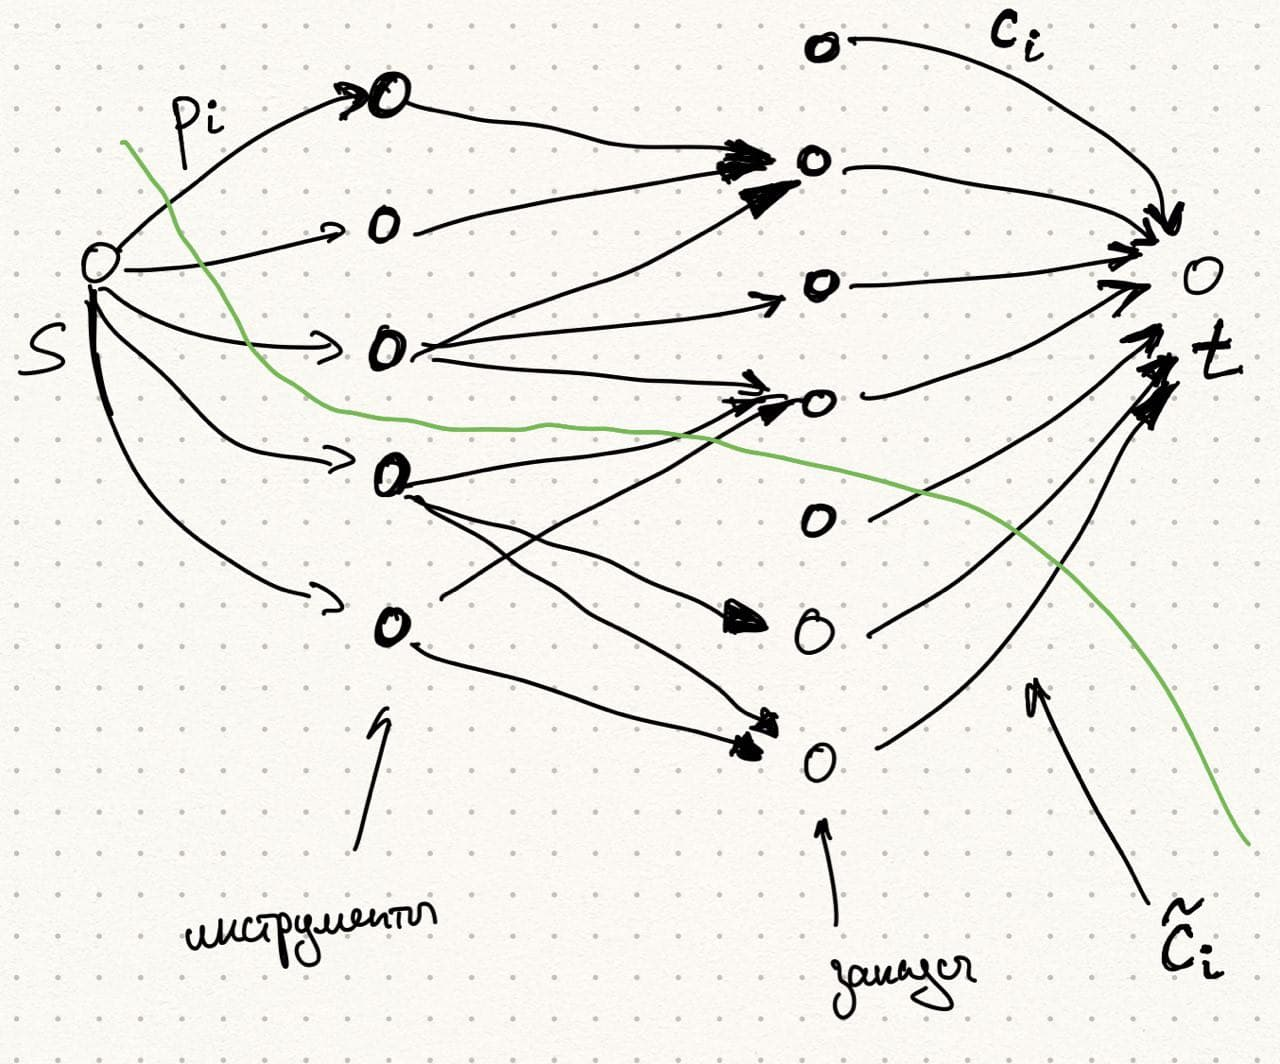
\includegraphics[width=0.5\textwidth]{pics/5.jpg}
            \caption{Граф с разрезом (зеленая кривая). Из-за бесконечной пропускной способности ребер между слоями они не проходят через разрез (на картинке проходят, но не должны)}
        \end{figure}
        Рассмотрим баланс в таком графе:
        \begin{equation}
            \sum c_i - \sum p_i = C - \underbrace{(\sum\tilde{c}_i + \sum p_i)}_{C(s,t)} \Longrightarrow \sum \tilde{c}_i + \sum p_i \to \min,
        \end{equation}
        где $C$ --- сумма вообще всех $c_i$, а $C(s,t)$ --- величина разреза.

        Теперь находим минимальный по величине разрез, тогда и прибыль максимизируется.
        \item Still pending.
    \end{enumerate}
\end{solution}